\section{Introduction}
\label{sec:introduction}

%\subsection{outline}
%
%KV is an important infrastructure service
%
%Existing solution of key-value store in
%
%1. CPU-based
%
%2. RDMA-based
%
%recent trend of programmable NIC in datacenter
%
%we present KV-Direct... 
%
%highlight the high level insight (offload the simple and performance critical operation to programmable NIC) 
%
%and design goal and spotlight (not only match the state of art of RDMA-based solution in GET operation and significant improve the PUT operation to even comparable to CPU-based solution. Moreover, our solution is more power and cost effective. With more FPGA or the improvement of FPGA, we can beat all existing CPU/RDMA solution.)
%
%KV-Direct makes contributions in three main aspects:
%
%1. proposes a KV solution for programmable NIC to Direct Memory Access.
%
%2. extends RDMA primitives to Key-value operation with consistency guarantee while high performance. 
%
%3. makes critical PCIe traffic optimization in our novel FPGA-based NIC key-value service design.



%Key-value store (KVS) is an infrastructure service to store shared structured data in a distributed system.
%Traditionally, the performance of KVS is mostly constrained by the OS network stack.
%Recent research leverage two-sided RDMA to accelerate communication among clients and KVS servers.
%The next bottleneck is CPU. The KV operation throughput of a CPU core is constrained by its latency hiding efficiency and computation capacity.
%Another approach is to use one-sided RDMA to bypass remote CPU and move KV processing to clients, but it incurs high communication and synchronization overhead.
%\subsection{current version}



\begin{figure*}[t]
\centering
\subfloat[Software / two-sided RDMA.\label{fig:memaccess-a}]
{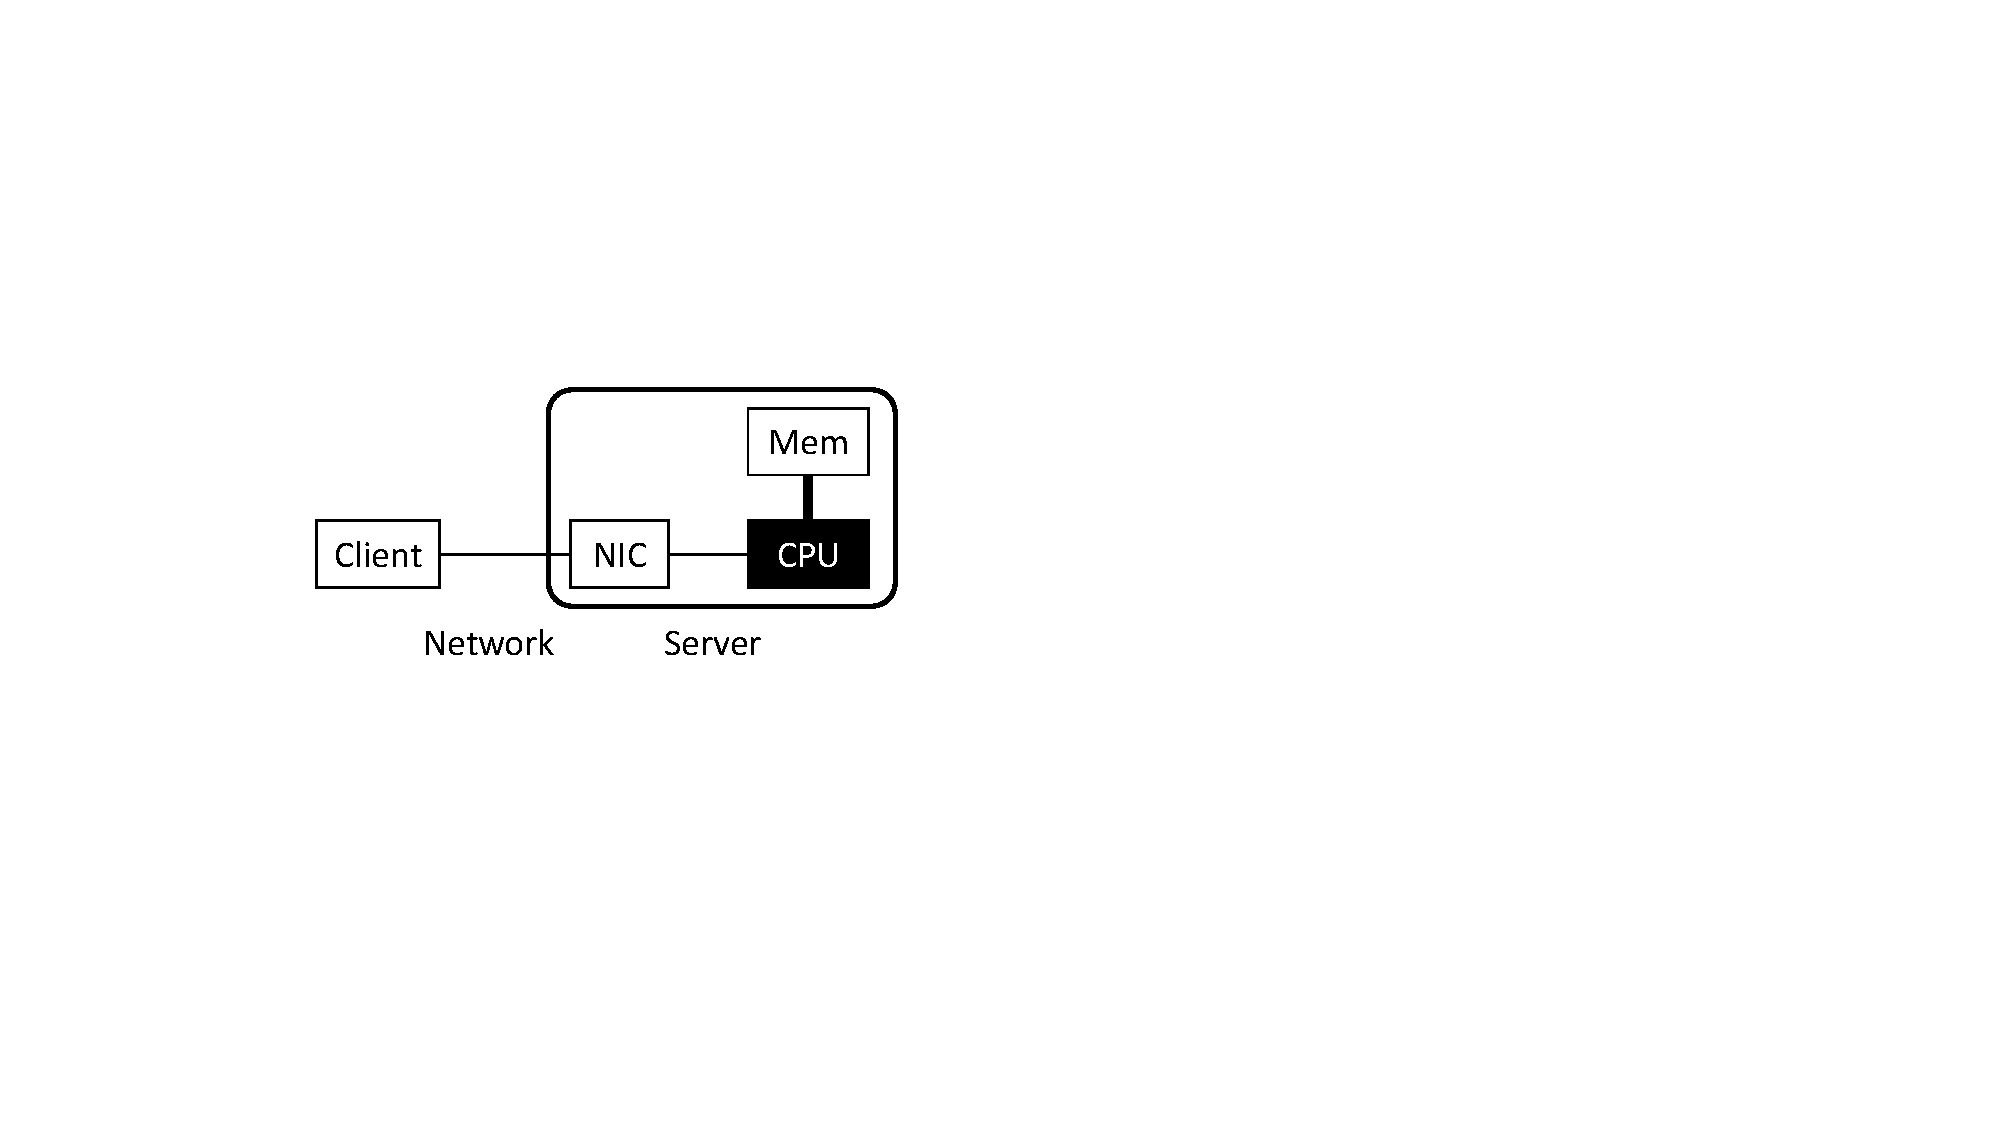
\includegraphics[width=.3\textwidth,page=1]{cropped_access.pdf}}
\subfloat[One-sided RDMA.\label{fig:memaccess-b}]
{\includegraphics[width=.3\textwidth,page=2]{cropped_access.pdf}}
\subfloat[KV-Direct.\label{fig:memaccess-c}]
{\includegraphics[width=.3\textwidth,page=3]{cropped_access.pdf}}
\caption{Design space of KVS data path and processing device. Line indicates data path. One KV operation (thin line) may require multiple address-based memory accesses (thick line). Black box indicates where KV processing takes place.}
\label{fig:memaccess}
\vspace{-10pt}
\end{figure*}

In-memory key-value store (KVS) is a key distributed system component in many data centers. KVS enables access to a shared key-value hash table among distributed clients. Historically, KVS such as Memcached~\cite{fitzpatrick2004distributed} gained popularity as an object caching system for web services. Large web service providers such as  Amazon~\cite{decandia2007dynamo} and Facebook~\cite{atikoglu2012workload, nishtala2013scaling}, have deployed distributed KVSs at scale. More recently, as main-memory based computing becomes a major trend in the data centers~\cite{ousterhout2010case,dragojevic2014farm}, KVS starts to go beyond caching and becomes an infrastructure to store shared data structure in a distributed system.
Many data structures can be expressed in a key-value hash table, \eg, data indexes in NoSQL databases~\cite{chang2008bigtable}, model parameters in machine learning~\cite{li2014scaling}, nodes and edges in graph computing~\cite{shao2013trinity, xiao17tux2} and sequencers in distributed synchronization~\cite{kalia2016design}. For most of these applications, the performance of the KVS is the key factor that directly determines the system efficiency. Due to its importance, over the years significant amount of research effort has been invested on improving KVS performance. 

Earlier key-value systems~\cite{decandia2007dynamo, fitzpatrick2004distributed, nishtala2013scaling} are built on top of traditional OS abstractions such as OS lock and TCP/IP stack. This puts considerable stress on the performance of the OS, especially the networking stack. The  bottleneck is exacerbated by the fact that physical network transport speed has seen huge improvements in the last decade due to heavy bandwidth demand from data center applications. 

More recently, as both the single core frequency scaling and multi-core architecture scaling are slowing down~\cite{sutter2005free,esmaeilzadeh2011dark}, a new research trend in distributed systems is to leverage Remote Direct Memory Access (RDMA) technology on NIC to reduce network processing cost. One line of research~\cite{kalia2014using, kalia2016design} uses two-sided RDMA to accelerate communication (Figure~\ref{fig:memaccess-a}). KVS built with this approach are bounded by CPU performance of the KVS servers. Another line of research uses one-sided RDMA to bypass remote CPU and shift KV processing workload to clients~\cite{dragojevic2014farm, mitchell2013using} (Figure~\ref{fig:memaccess-b}). This approach achieves better GET performance but degrades performance for PUT operations due to high communication and synchronization overhead. It is evident that the limited abstraction provided by RDMA is not a perfect fit for building efficient KVS. 

In the meantime, another trend is emerging in data center hardware evolution. More and more servers in data centers are now equipped with \ournic{}s~\cite{caulfield2016cloud, greenberg2015sdn,putnam2014reconfigurable}.
At the heart of a programmable NIC is a field-programmable gate array (FPGA) with an embedded NIC chip to connect to the network and a PCIe connector to attach to the server.
Programmable NIC is initially designed to enable network virtualization~\cite{vfp,li2016clicknp}.
However, many found that FPGA resources can be used to offload some workloads of CPU and significantly reduce CPU resource usage~\cite{ouyang14hotchips, MaZC17fpga, huang16socc, cong16dac}. Our work takes this general approach.

We present \oursys{}, a new in-memory key-value system that takes advantage of \ournic{} in data center.
\oursys{}, as its name implies, directly fetches data and applies updates in the host memory to serve KV requests, bypassing host CPU (Figure~\ref{fig:memaccess-c}).
%We leverage the insight of one-sided RDMA-based KV systems to bypass CPU, while offload the computation logic to FPGA-based NIC to ensure the consistency in server side, which results in the remarkable performance improvement through network traffic reduction and less synchronization overhead, furthermore, the client side becomes transparent to all KV operations.
\oursys{} extends the RDMA primitives from memory operations (READ and WRITE) to key-value operations (GET, PUT, DELETE and ATOMIC ops). Compared with one-sided RDMA based systems, \oursys{} deals with the consistency and synchronization issues at server-side, thus remove the computation load in client and reduce network traffic.
In addition, to support vector-based operations and reduce network traffic, \oursys{} also provides new vector primitives UPDATE, REDUCE, and FILTER, allowing users to define active messages~\cite{eicken1992active} and delegate certain computation to programmable NIC for efficiency.

Since the key-value operations are offloaded to the \ournic{}, we focus our design on optimizing the PCIe traffic between the NIC and host memory. \oursys{} adopts a series of optimizations to fully utilizing PCIe bandwidth and hide latency. Firstly, we design a new hash table and memory allocator to leverage parallelism available in FPGA and minimize the number of PCIe DMA requests. On average, \oursys{} achieves close to one PCIe DMA per READ operation and two PCIe DMAs per WRITE operation. Secondly, to guarantee consistency among dependent KV operations, \oursys{} includes an out-of-order execution engine to track operation dependencies while maximizing the throughput of independent requests. Thirdly, \oursys{} exploits on-board DRAM buffer available on \ournic{} by implementing a hardware-based load dispatcher and caching component in FPGA to fully utilize on-board DRAM bandwidth and capacity. 

%%\textbf{TODO:performance highlight}
%three key results:
%
A single NIC \oursys{} is able to achieve up to 180~M KV operations per second (Ops), equivalent to the throughput of 36 CPU cores~\cite{li2016full}. Compared with state-of-art CPU KVS implementations, \oursys{} reduces tail latency to as low as 10~\mus{} while achieving a 10\approx20x improvement on power efficiency. Moreover, \oursys{} can achieve near linear scalability with multiple NICs. With 8 \ournic{} cards in a server we achieve one billion KV operations per second per server node, which is more than an order of magnitude improvement over existing systems.

\oursys{} supports general atomic operations up to 180~Mops, equal to normal KV operation and significantly outperforms the number reported in state-of-art RDMA-based system: 2.24~Mops~\cite{kalia2014using}. The atomic operation agnostic performance is mainly a result of our out-of-order execution engine that can efficiently track the dependency among KV operations without explicitly stalling the pipeline.

%The rest of the paper is organized as follows. \S\ref{sec:background} shows the background, clarifies our design goals as well as challenges. \S\ref{sec:architecture} describes \oursys{} design. \S\ref{sec:implementation} presents the implementation details of \oursys{}. \S\ref{sec:evaluation} is the evaluation of \oursys{}. \S\ref{sec:extensions} talks about the further extensions. We discuss the related work in \S\ref{sec:related} and conclude in \S\ref{sec:conclusion}.
